\documentclass{beamer}

\usetheme{Gelugor}

\usepackage{graphicx} 
\usepackage{booktabs} 
\usepackage{lmodern}
\usepackage[utf8]{inputenc} 
\usepackage[czech]{babel} 
\usepackage{amsmath}
\usepackage{amssymb}
\usepackage{amsthm}
\usepackage{pifont}
\usepackage{xcolor}
\usepackage{bm}
\usepackage{listings}
\usepackage{tabularx} 
\usepackage{textpos}


\renewcommand{\lstlistingname}{Ukázka}
\theoremstyle{definition}
\newtheorem{definice}{Definice shrinku}

% \AtBeginSection[]
% {
%    \begin{frame}
%        \frametitle{Obsah}
%        \vspace{2em}
%        \tableofcontents[currentsection, subsubsectionstyle={show/show/show/shaded}
%        ]
%    \end{frame}
% }

%----------------------------------------------------------------------------------------

% \title{\textbf{UML}} 
\author[Bc. Anna Gruberová]{Vypracovala: Bc. Anna Gruberová  \linebreak  Vedoucí práce: Ing. Martin Plajner, Ph.D.}
\institute[]{Fakulta jaderná a fyzikálně inženýrská ČVUT v Praze}
\date{11. dubna 2022}
\title{Analýza příčin vzniku shrinku produktů společnosti na základě logistických dat}
\subtitle{Diplomová práce}


\begin{document}
{
  \begin{frame}[plain]
	\vspace{0.8cm}
    \titlepage 
	\vspace{-0.8cm}
	
    \end{frame}
}
    
\begin{frame}
  \frametitle{Obsah}
  \tableofcontents
\end{frame}

\section{Motivace a cíle práce}
   
% \begin{frame}
%     \frametitle{Motivace a cíle práce}

% \end{frame}


\section{Teoretická část}
   
\begin{frame}
    \frametitle{Popis úlohy}
	\begin{itemize}
    	\item Z obdržených dat analyzovat přičiny vzniku shrinku produktů
    	\item[] (předpovědět typ a množství).
    \end{itemize}

	\begin{definice}
		\textbf{Ztráta zisku z neuskutečněného prodeje hotového produktu.}
		\begin{itemize}
			\item[ -]Produkt je vyroben (naskladněn), ale nebyl prodán zákazníkovi. 
			\item[ -]Důvody: poničení, ztráta nebo prošlá doba spotřeby aj. 
		\end{itemize}
	\end{definice}
	
	% Za shrink produktu lze označovat i stav, kdy cena produktu je neplánovaně snížena v důsledku zmíněných důvodů. Shrinkem je potom rozdíl plánované prodejní ceny a ceny, za kterou byl produkt skutečně prodán.
    \begin{itemize}
    	\item 
    \end{itemize}

\end{frame}


\section{Vybrané metody a datové sady}
 

% \begin{frame}
%     \frametitle{Testované metody}
%     \begin{itemize}
%     	\item 
%     \end{itemize}
% \end{frame}

\section{Postup implementace}

\begin{frame}
    \frametitle{Postup zpracování úlohy}
	\vspace{0.7cm}
	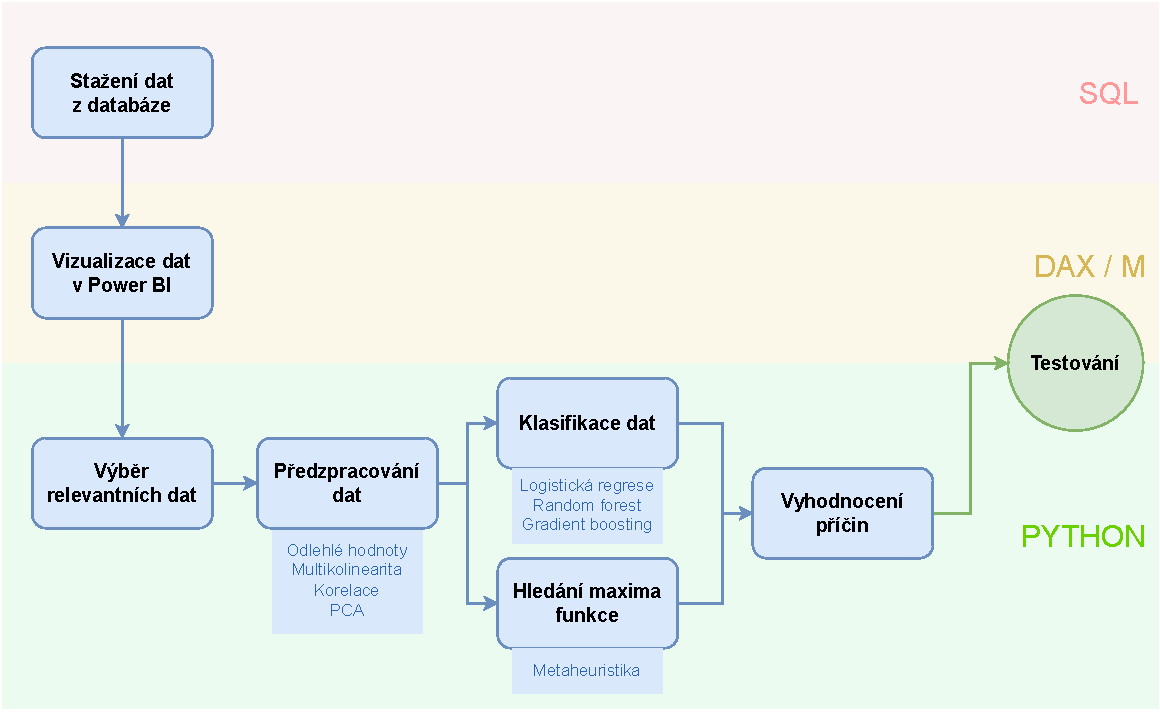
\includegraphics[width=\textwidth]{pipelineDP.drawio.pdf}
\end{frame}

\section{Výsledky}
   

\begin{frame}
    \frametitle{Výsledky}
	\begin{itemize}
    	\item 
    \end{itemize}
	\resizebox{\textwidth}{!}{%
	\begin{tabular}{lcc}
		Metoda                          & Přesnost (trénovací data) & Přesnost (testovací data) \\ \hline
		Logistická regrese OVR          & 77,04 \%                  & 76,95 \%                  \\
		Multinomická logistická regrese & 77,33 \%                  & 77,27 \%                  \\
		Random forest                   & 82,54 \%                  & 82.12 \%                  \\      
		\textbf{Gradient boosting}               & \textbf{83,80 \% }                 & \textbf{83,78 }\%               
		\end{tabular}
	}
	
    % \includegraphics[width=\textwidth]{grafy/resCTW.png}

\end{frame}



\begin{frame}
    \Large{\centerline{Děkuji za pozornost.}}
\end{frame}

\end{document}